\section{项目成果与功能验证}

\subsection{开发与实验环境}
项目在 Windows 上开发，采用 HTML、CSS 和 JavaScript 编写应用内页面，由 Android WebView 加载。页面通过 Java 原生桥接访问外部服务，原生层负责会话管理，返回的数据由页面整理和展示。应用的安装、启动和页面交互在 MuMu 的 Android 15 环境中检验。实验分为实际账户查询、本机操作和合成输入检查。实际账户查询用于核对服务能否返回可用结果，本机操作用于检查界面和数据保存，合成输入用于验证阈值、筛选及异常处理等可控条件。图示采用当前版本的运行画面，保留了对早期业务实验结果的独立说明。

\subsection{主要界面与运行成果}
上一章图\ref{fig:beforeafter}已展示新版课表操作区。图\ref{fig:run-main}进一步展示学习入口与待办操作区。待办界面可见实际输入区、状态筛选和已有测试事项，学习截图使用未连接的测试账户。图\ref{fig:run-other}把生活入口与统一账号列表相邻呈现。饮水页提供登录入口，账号列表呈现五项服务各自的状态。“我的”仍设有外观与缓存管理。生活页与账号中心同样使用未授权的测试账户，展示的是接入入口与连接状态。

\begin{figure}[!htb]
\centering
\begin{tabular}[t]{@{}c@{\hspace{5mm}}c@{}}
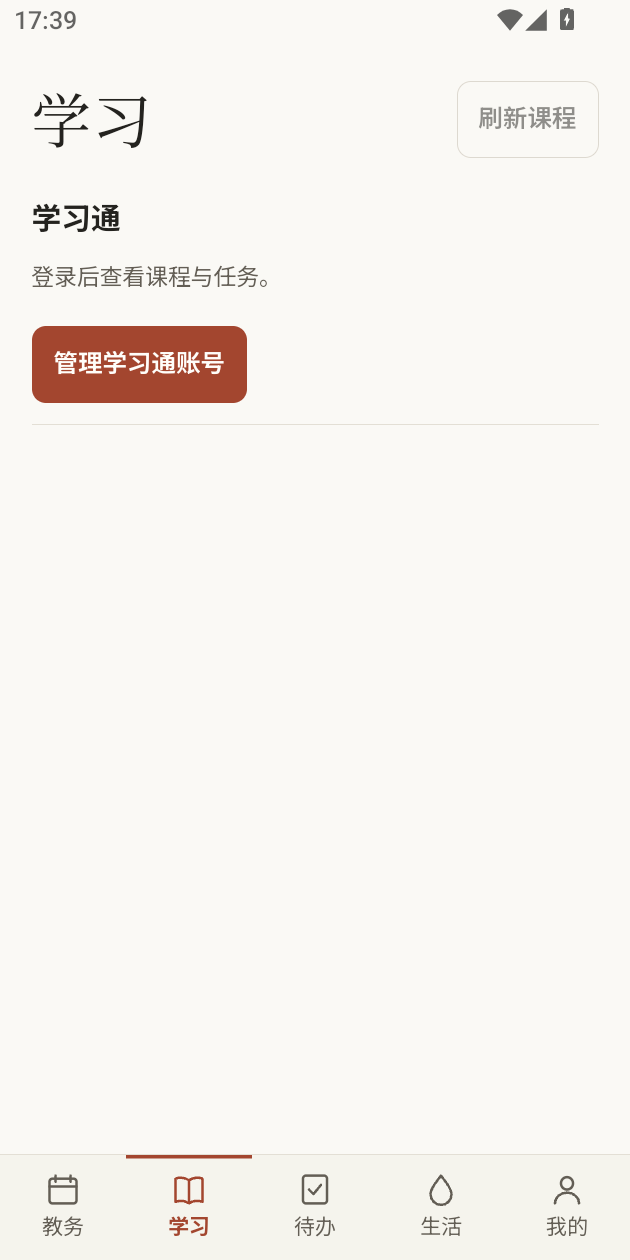
\includegraphics[width=.46\linewidth,trim=0bp 585bp 0bp 34bp,clip]{after-study.png} &
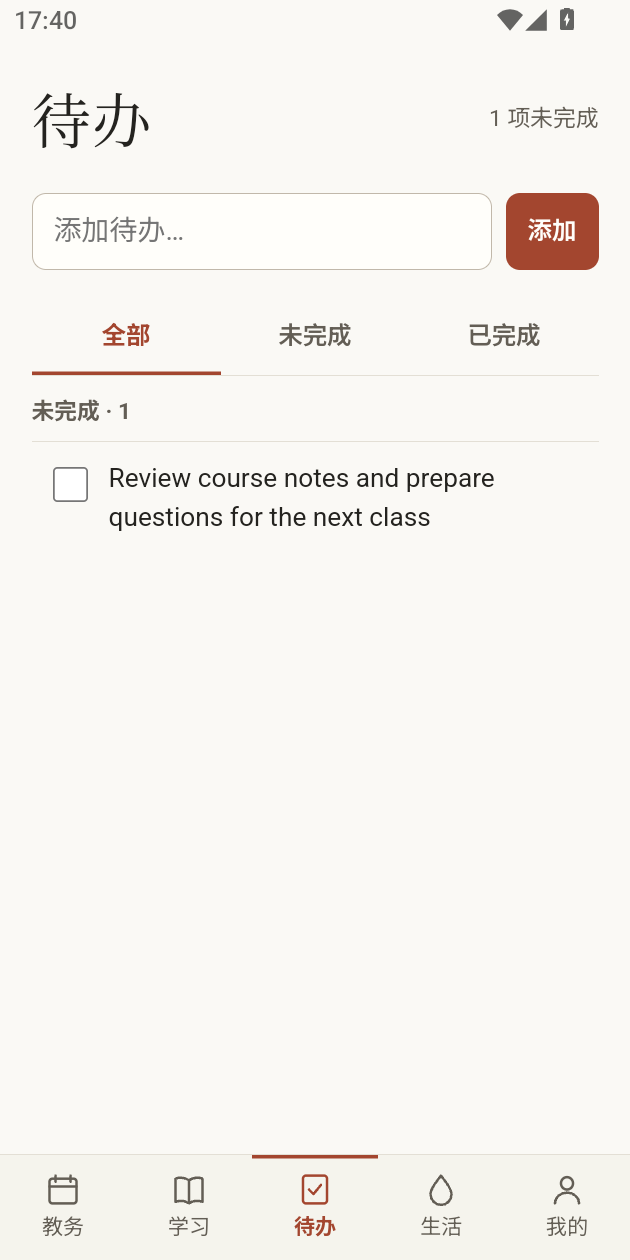
\includegraphics[width=.46\linewidth,trim=0bp 585bp 0bp 34bp,clip]{after-todo.png} \\
\small （a）学习入口 & \small （b）本地待办
\end{tabular}
\caption{学习入口与本地待办的实际操作区域}\label{fig:run-main}
\end{figure}

\begin{figure}[!htb]
\centering
\begin{tabular}[t]{@{}c@{\hspace{5mm}}c@{}}
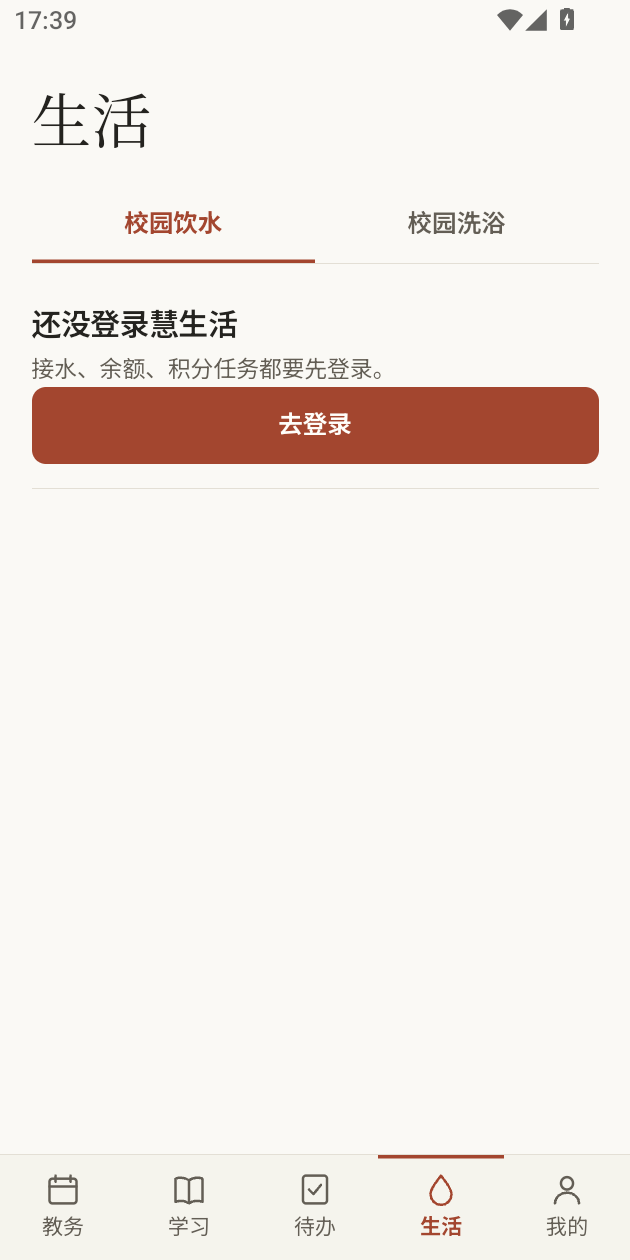
\includegraphics[width=.46\linewidth,trim=0bp 466bp 0bp 34bp,clip]{after-life.png} &
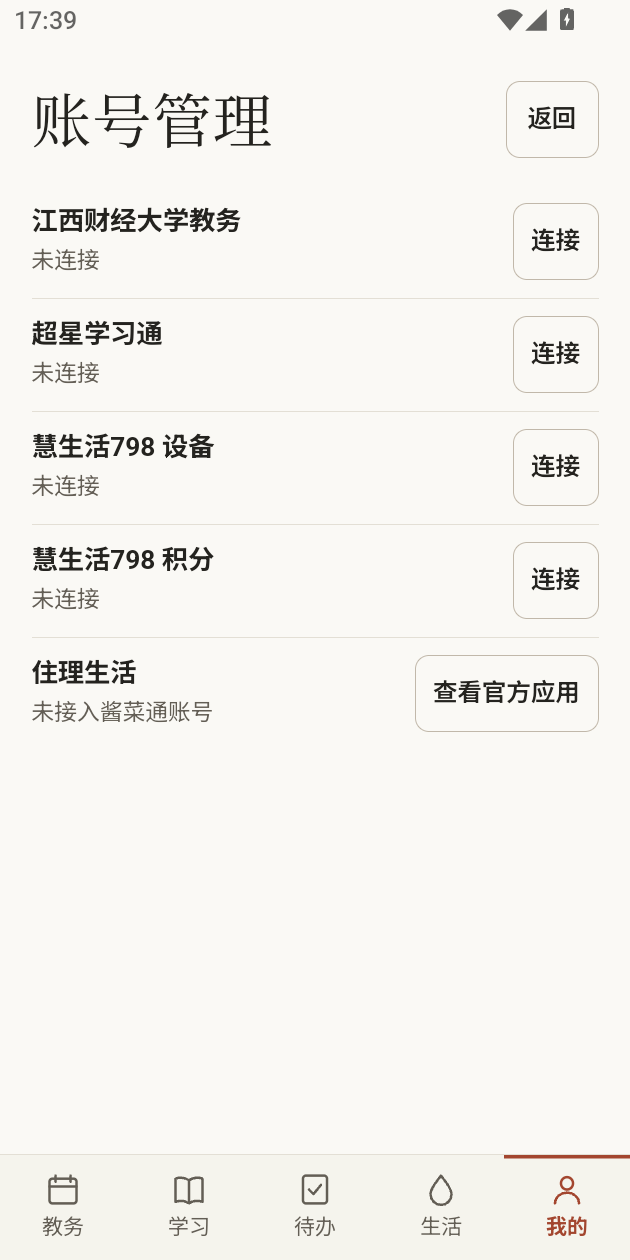
\includegraphics[width=.46\linewidth,trim=0bp 466bp 0bp 34bp,clip]{after-accounts.png} \\
\small （a）生活入口 & \small （b）统一账号管理
\end{tabular}
\caption{生活入口与“我的”账号中心的实际界面}\label{fig:run-other}
\end{figure}

\subsection{典型操作流程}
\textbf{教务查询}\quad 首次从账号中心发起校方登录，然后在教务页选择学期和周次。应用按账号和学期读取本机结果，确认可访问时再读取校方个人课表。课程块可查看详细地点及周次。已验证 261、252 学期的真实课表读取，当前版本重新启动后仍可回读已保存的课表。

\textbf{学习任务}\quad 有效会话下进入学习页，按当前教学班读取或刷新。作业、考试和活动经解析归并，用户从类型与状态筛选切换至按课程查看，再决定是否打开任务链接。实际扫描及教学班分组已通过真实课程检验，窄屏上的筛选和分组另用本地合成任务复核。

\textbf{本地待办}\quad 输入一项任务并添加，打开详情编辑备注，随后勾选完成并从相应筛选项检查结果。用户可取消完成，也可二次确认删除。模拟器中的操作覆盖新增、编辑、筛选、勾选和删除。重新加载后，已保存的记录可以恢复。

\textbf{饮水查询}\quad 设备账号本人验证成功后，返回生活页查看余额、收藏设备与消费账单。真实账户实验核对了这三项结果，重新启动应用后也可再次查询。新版页面复核覆盖了饮水入口和账号界面。

\subsection{实验结果与分析}
表\ref{tab:validation}汇总了主要实验及其运行结果。课表、成绩、学习任务和用水账户的真实查询检验了应用与各服务的数据交互。界面操作和合成输入分别用于验证日常操作及边界行为。考试开放批次返回了空报表，住理生活原生功能也尚未取得真实业务结果，两者的验证范围在表中单列说明。

\begin{table}[htbp]
\centering\small
\caption{主要功能的测试内容与运行结果}\label{tab:validation}
\begin{tabularx}{\linewidth}{@{}>{\raggedright\arraybackslash}p{24mm}>{\raggedright\arraybackslash}p{43mm}Y@{}}
\toprule
功能模块 & 测试内容 & 运行结果 \\
\midrule
教务 & 真实课表读取、静默刷新、成绩切换与缓存回读 & 课表可读取并更新，四个成绩学期可切换。考试开放批次仅返回真实空报表，非空记录解析待核查。 \\
学习通 & 实际课程扫描、课程分组、隐藏课程复查及筛选 & 实际读取课程及任务，隐藏项可参与复查。筛选和自动恢复规则另经合成检查，长期恢复仍待观测。 \\
本地待办 & 新增、编辑、勾选、筛选、删除及重启 & 模拟器操作通过，已保存记录可恢复。带可见软键盘的遮挡情况仍待设备复核。 \\
慧生活798 & 设备账号登录及重启后查询 & 实际读取余额、收藏设备和账单。积分登录、兑换及设备启停待验证。 \\
住理生活 & 官方应用入口、设备选择页及连接状态 & 可打开官方入口，已观察设备选择页。本机状态处理经合成检查，原生查询与控制仍待接入。 \\
导航与账号 & 安装启动、服务入口、主题切换 & 五项导航和账号入口可用，深浅主题可切换。界面检查覆盖当前版本，线上查询结论来自前述业务实验。 \\
\bottomrule
\end{tabularx}
\end{table}
